\documentclass[11pt,]{article}
\usepackage[left=1in,top=1in,right=1in,bottom=1in]{geometry}
\newcommand*{\authorfont}{\fontfamily{phv}\selectfont}
\usepackage[]{mathpazo}


  \usepackage[T1]{fontenc}
  \usepackage[utf8]{inputenc}



\usepackage{abstract}
\renewcommand{\abstractname}{}    % clear the title
\renewcommand{\absnamepos}{empty} % originally center

\renewenvironment{abstract}
 {{%
    \setlength{\leftmargin}{0mm}
    \setlength{\rightmargin}{\leftmargin}%
  }%
  \relax}
 {\endlist}

\makeatletter
\def\@maketitle{%
  \newpage
%  \null
%  \vskip 2em%
%  \begin{center}%
  \let \footnote \thanks
    {\fontsize{18}{20}\selectfont\raggedright  \setlength{\parindent}{0pt} \@title \par}%
}
%\fi
\makeatother




\setcounter{secnumdepth}{0}


\usepackage{graphicx,grffile}
\makeatletter
\def\maxwidth{\ifdim\Gin@nat@width>\linewidth\linewidth\else\Gin@nat@width\fi}
\def\maxheight{\ifdim\Gin@nat@height>\textheight\textheight\else\Gin@nat@height\fi}
\makeatother
% Scale images if necessary, so that they will not overflow the page
% margins by default, and it is still possible to overwrite the defaults
% using explicit options in \includegraphics[width, height, ...]{}
\setkeys{Gin}{width=\maxwidth,height=\maxheight,keepaspectratio}

\title{ChangeMyView: How Moral Appeals Induce Persuasion  }



\author{\Large Patrick W. Kraft\vspace{0.05in} \newline\normalsize\emph{Stony Brook University}  }


\date{}

\usepackage{titlesec}

\titleformat*{\section}{\normalsize\bfseries}
\titleformat*{\subsection}{\normalsize\itshape}
\titleformat*{\subsubsection}{\normalsize\itshape}
\titleformat*{\paragraph}{\normalsize\itshape}
\titleformat*{\subparagraph}{\normalsize\itshape}





\newtheorem{hypothesis}{Hypothesis}
\usepackage{setspace}

\makeatletter
\@ifpackageloaded{hyperref}{}{%
\ifxetex
  \PassOptionsToPackage{hyphens}{url}\usepackage[setpagesize=false, % page size defined by xetex
              unicode=false, % unicode breaks when used with xetex
              xetex]{hyperref}
\else
  \PassOptionsToPackage{hyphens}{url}\usepackage[unicode=true]{hyperref}
\fi
}

\@ifpackageloaded{color}{
    \PassOptionsToPackage{usenames,dvipsnames}{color}
}{%
    \usepackage[usenames,dvipsnames]{color}
}
\makeatother
\hypersetup{breaklinks=true,
            bookmarks=true,
            pdfauthor={Patrick W. Kraft (Stony Brook University)},
             pdfkeywords = {Moral Foundations, Persuasion, Attitude Change},  
            pdftitle={ChangeMyView: How Moral Appeals Induce Persuasion},
            colorlinks=true,
            citecolor=blue,
            urlcolor=blue,
            linkcolor=magenta,
            pdfborder={0 0 0}}
\urlstyle{same}  % don't use monospace font for urls

% set default figure placement to htbp
\makeatletter
\def\fps@figure{htbp}
\makeatother



% add tightlist ----------
\providecommand{\tightlist}{%
\setlength{\itemsep}{0pt}\setlength{\parskip}{0pt}}

\begin{document}
	
% \pagenumbering{arabic}% resets `page` counter to 1 
%
% \maketitle

{% \usefont{T1}{pnc}{m}{n}
\setlength{\parindent}{0pt}
\thispagestyle{plain}
{\fontsize{18}{20}\selectfont\raggedright 
\maketitle  % title \par  

}

{
   \vskip 13.5pt\relax \normalsize\fontsize{11}{12} 
\textbf{\authorfont Patrick W. Kraft} \hskip 15pt \emph{\small Stony Brook University}   

}

}








\begin{abstract}

    \hbox{\vrule height .2pt width 39.14pc}

    \vskip 8.5pt % \small 

\noindent Overview of initial results


\vskip 8.5pt \noindent \emph{Keywords}: Moral Foundations, Persuasion, Attitude Change \par

    \hbox{\vrule height .2pt width 39.14pc}



\end{abstract}


\vskip 6.5pt


\noindent  \section{Introduction}\label{introduction}

\section{Description of Dataset}\label{description-of-dataset}

\section{\texorpdfstring{\emph{ToDos}}{ToDos}}\label{todos}

\begin{itemize}
\tightlist
\item
  clean original posts (links etc)!
\item
  adjust confidence intervals to correct for multiple comparisons
\item
  add more comments in functions!
\end{itemize}

\section{Moral Foundations and
Persuadability}\label{moral-foundations-and-persuadability}

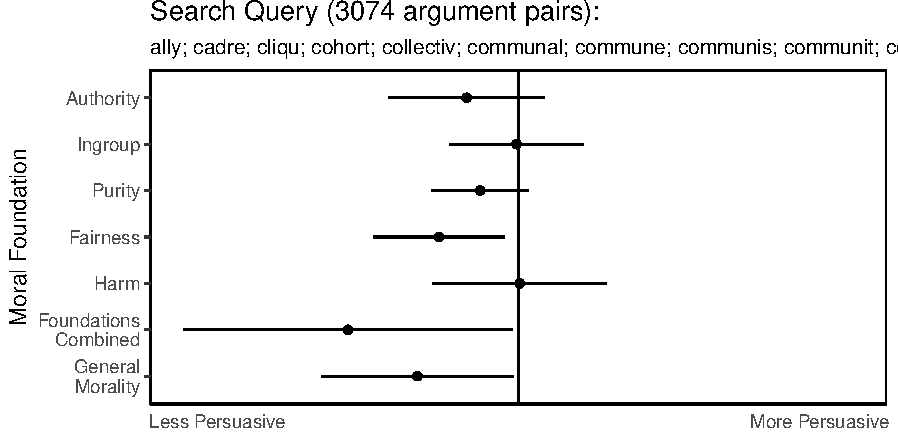
\includegraphics{prelim_files/figure-latex/unnamed-chunk-3-1.pdf}

\section{Is Moral Consistency
Convincing?}\label{is-moral-consistency-convincing}

\emph{Authority}

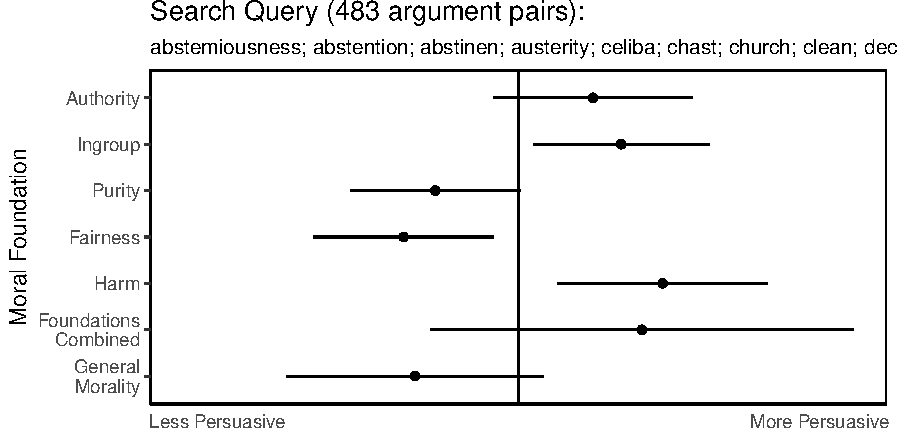
\includegraphics{prelim_files/figure-latex/unnamed-chunk-5-1.pdf}

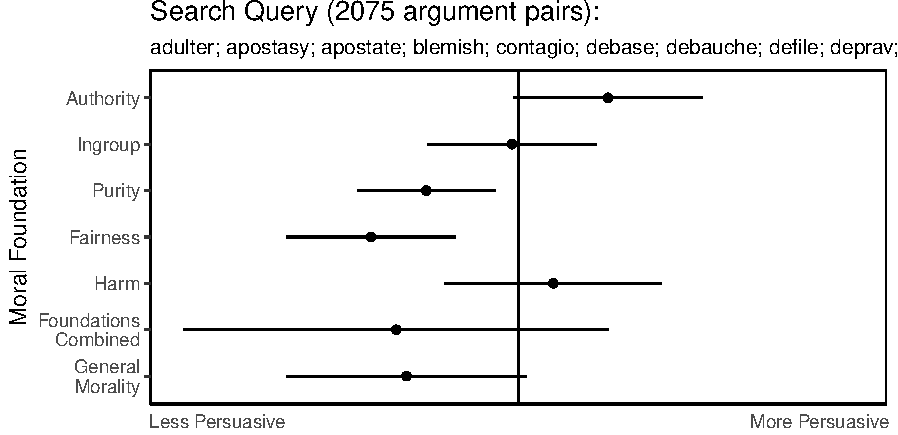
\includegraphics{prelim_files/figure-latex/unnamed-chunk-6-1.pdf}

\emph{Ingroup}

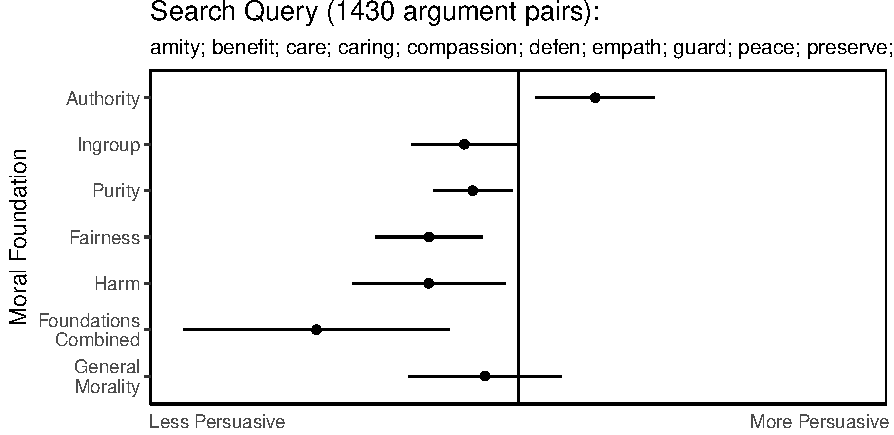
\includegraphics{prelim_files/figure-latex/unnamed-chunk-7-1.pdf}

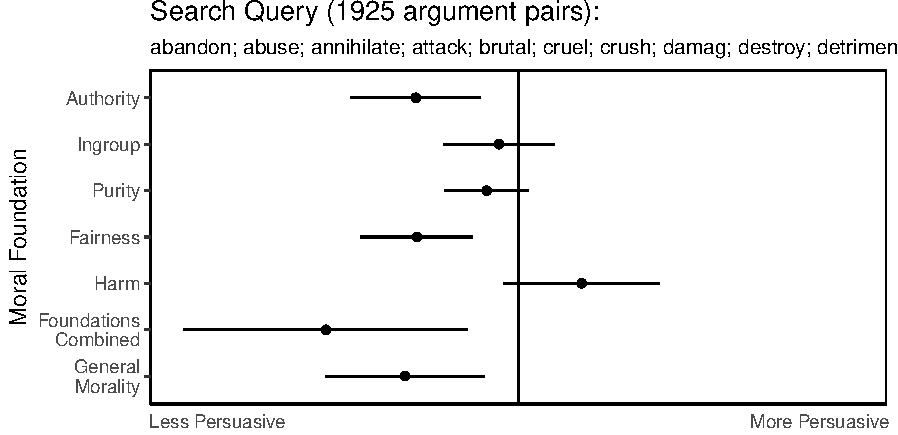
\includegraphics{prelim_files/figure-latex/unnamed-chunk-8-1.pdf}

\emph{Purity}

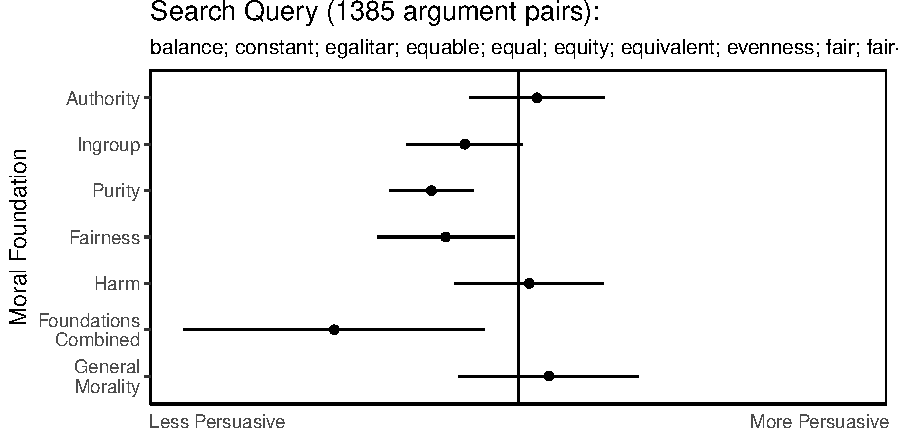
\includegraphics{prelim_files/figure-latex/unnamed-chunk-9-1.pdf}

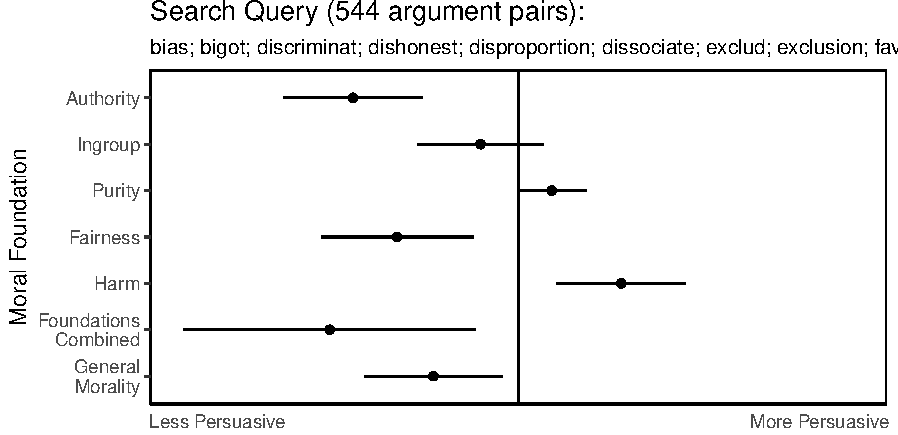
\includegraphics{prelim_files/figure-latex/unnamed-chunk-10-1.pdf}

\emph{Harm}

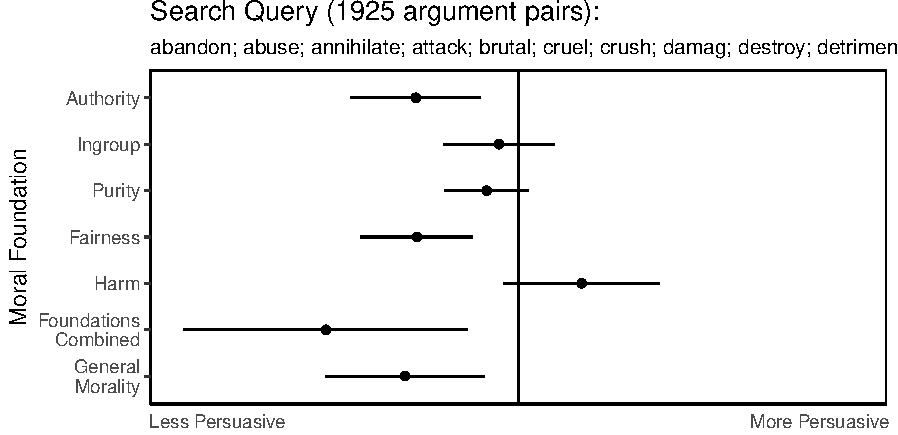
\includegraphics{prelim_files/figure-latex/unnamed-chunk-11-1.pdf}

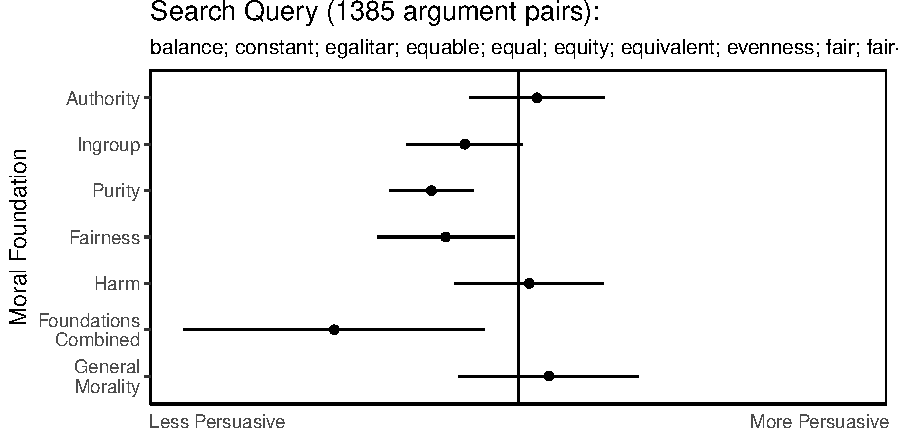
\includegraphics{prelim_files/figure-latex/unnamed-chunk-12-1.pdf}

\emph{Fairness}

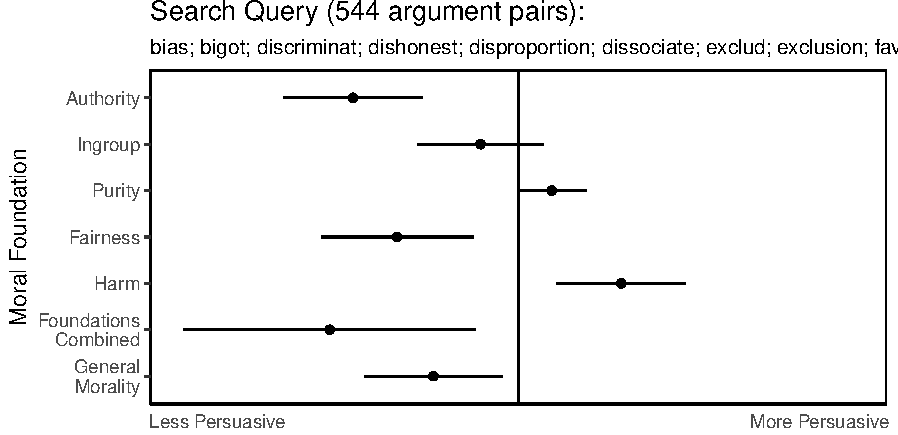
\includegraphics{prelim_files/figure-latex/unnamed-chunk-13-1.pdf}

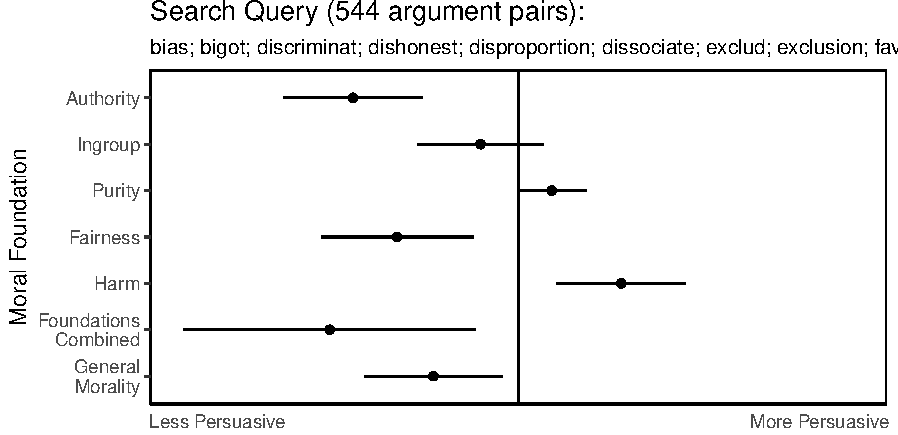
\includegraphics{prelim_files/figure-latex/unnamed-chunk-14-1.pdf}

\section{How about other topics?}\label{how-about-other-topics}

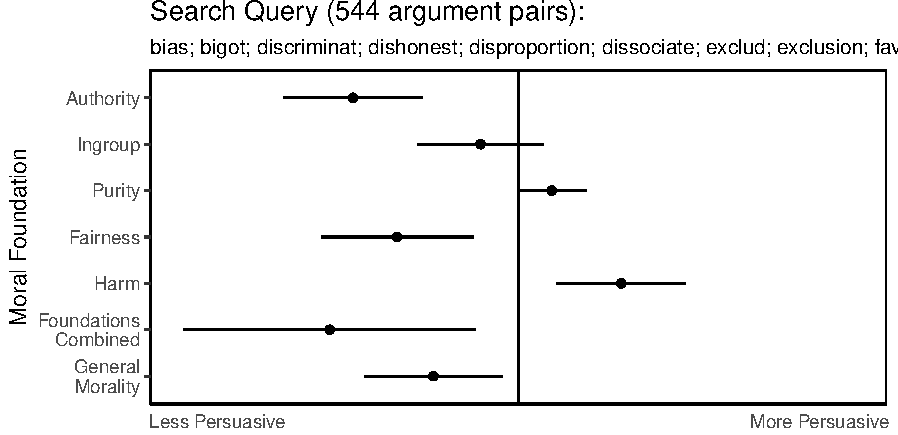
\includegraphics{prelim_files/figure-latex/unnamed-chunk-15-1.pdf}

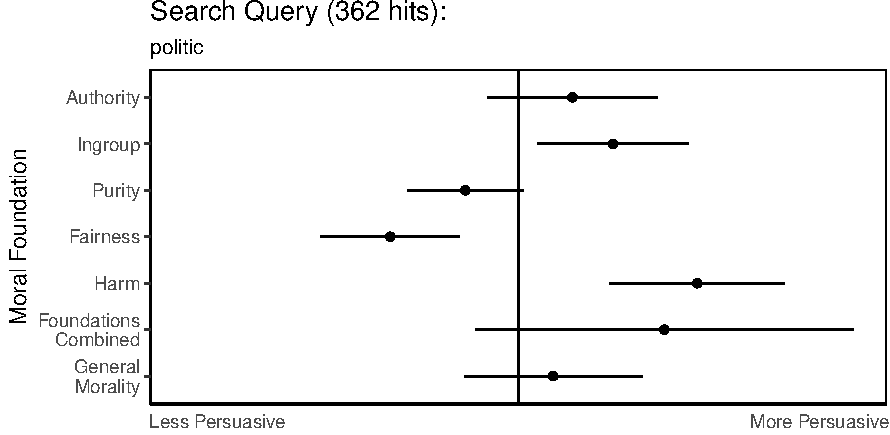
\includegraphics{prelim_files/figure-latex/unnamed-chunk-16-1.pdf}

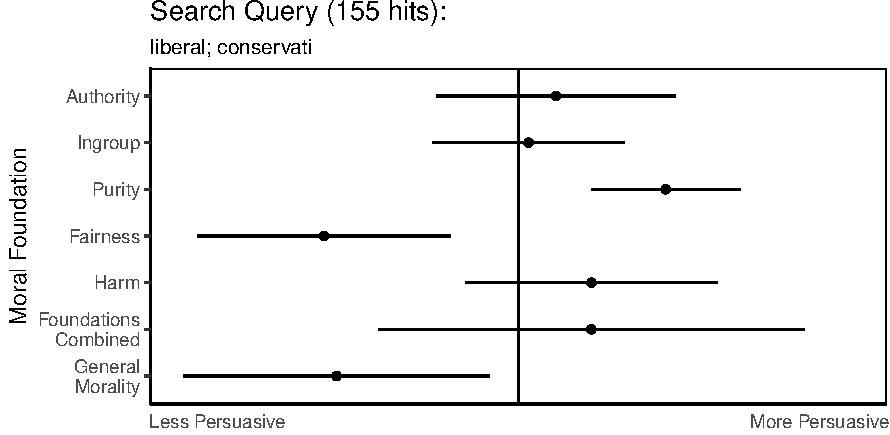
\includegraphics{prelim_files/figure-latex/unnamed-chunk-17-1.pdf}

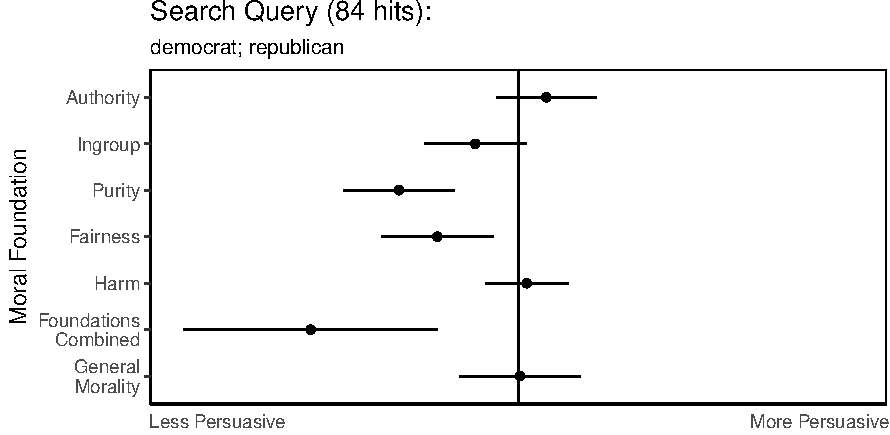
\includegraphics{prelim_files/figure-latex/unnamed-chunk-18-1.pdf}

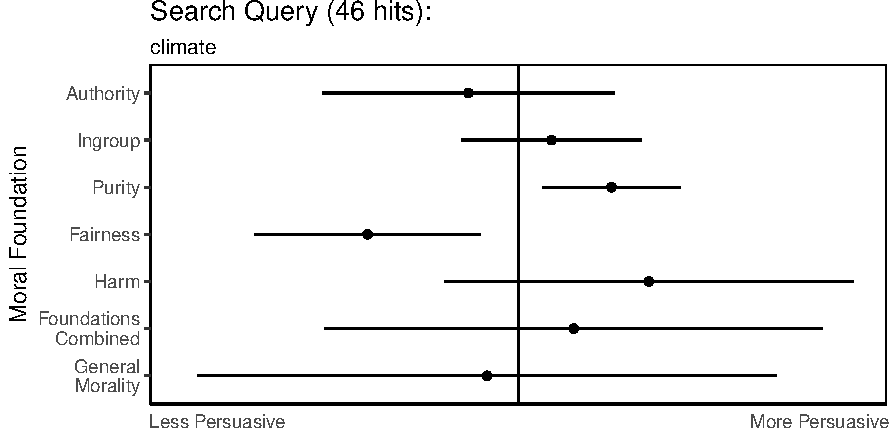
\includegraphics{prelim_files/figure-latex/unnamed-chunk-19-1.pdf}

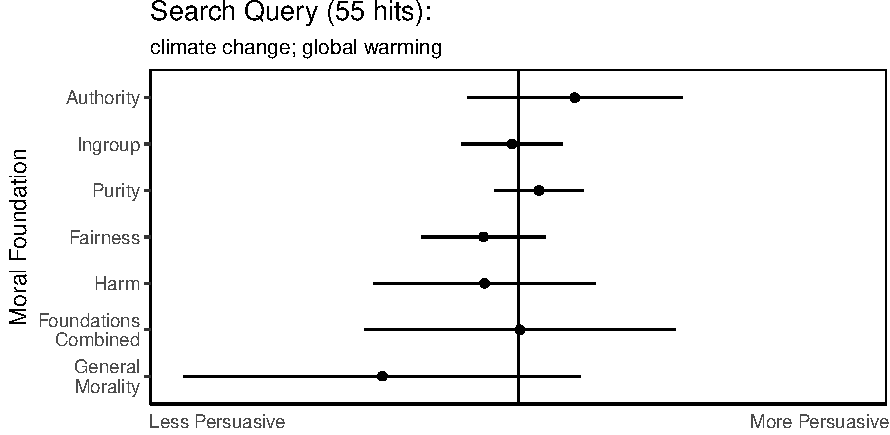
\includegraphics{prelim_files/figure-latex/unnamed-chunk-20-1.pdf}

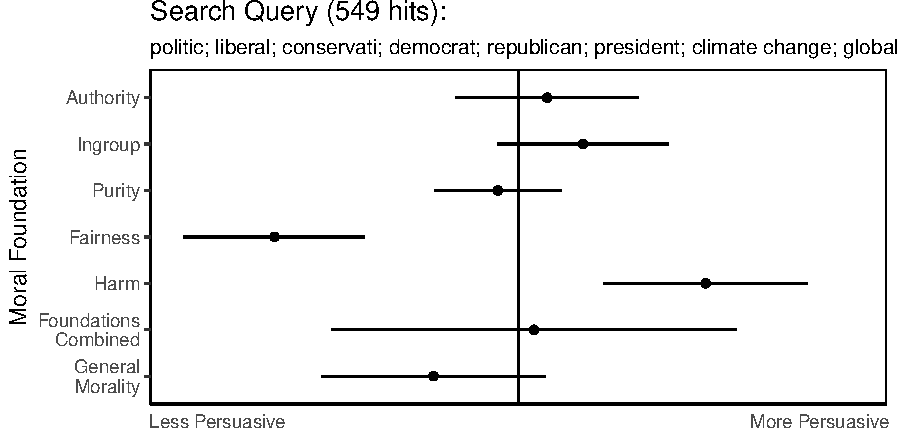
\includegraphics{prelim_files/figure-latex/unnamed-chunk-21-1.pdf}




\newpage
\singlespacing 
\end{document}
